
%(BEGIN_QUESTION)
% Copyright 2012, Tony R. Kuphaldt, released under the Creative Commons Attribution License (v 1.0)
% This means you may do almost anything with this work of mine, so long as you give me proper credit

This solar-powered pump system has a problem.  The pump motor is supposed to turn on according to a timed schedule set by the timer switch, yet the pump never comes on even when the sun is shining fully on the electricity-generating solar panels.  Each panel generates 22 volts when open-circuited (i.e. no load) and 15 volts when driving the pump motor:

$$\includegraphics[width=15.5cm]{i01141x01.eps}$$

A DC voltmeter connected between terminals 9 and 12 registers 0 volts when the sun is shining brightly and the timer switch is supposed to be in its ``on'' state to run the pump.  Identify the likelihood of each specified fault for this circuit.  Consider each fault one at a time (i.e. no coincidental faults), determining whether or not each fault could independently account for {\it all} measurements and symptoms in this circuit.

% No blank lines allowed between lines of an \halign structure!
% I use comments (%) instead, so that TeX doesn't choke.

$$\vbox{\offinterlineskip
\halign{\strut
\vrule \quad\hfil # \ \hfil & 
\vrule \quad\hfil # \ \hfil & 
\vrule \quad\hfil # \ \hfil \vrule \cr
\noalign{\hrule}
%
% First row
{\bf Fault} & {\bf Possible} & {\bf Impossible} \cr
%
\noalign{\hrule}
%
% Another row
Wire connecting terminals 8 and 9 failed open &  &  \cr
%
\noalign{\hrule}
%
% Another row
Wire connecting terminals 1 and 12 failed open &  &  \cr
%
\noalign{\hrule}
%
% Another row
Wire connecting terminal 5 to solar panel failed open &  &  \cr
%
\noalign{\hrule}
%
% Another row
Wire connecting terminals 10 and 11 failed open &  &  \cr
%
\noalign{\hrule}
%
% Another row
Timer switch failed shorted &  &  \cr
%
\noalign{\hrule}
%
% Another row
Timer switch failed open &  &  \cr
%
\noalign{\hrule}
%
% Another row
Fuse blown open &  &  \cr
%
\noalign{\hrule}
%
% Another row
Pump motor failed open &  &  \cr
%
\noalign{\hrule}
} % End of \halign 
}$$ % End of \vbox

\underbar{file i01141}
%(END_QUESTION)





%(BEGIN_ANSWER)

% No blank lines allowed between lines of an \halign structure!
% I use comments (%) instead, so that TeX doesn't choke.

$$\vbox{\offinterlineskip
\halign{\strut
\vrule \quad\hfil # \ \hfil & 
\vrule \quad\hfil # \ \hfil & 
\vrule \quad\hfil # \ \hfil \vrule \cr
\noalign{\hrule}
%
% First row
{\bf Fault} & {\bf Possible} & {\bf Impossible} \cr
%
\noalign{\hrule}
%
% Another row
Wire connecting terminals 8 and 9 failed open & $\surd$ &  \cr
%
\noalign{\hrule}
%
% Another row
Wire connecting terminals 1 and 12 failed open & $\surd$ &  \cr
%
\noalign{\hrule}
%
% Another row
Wire connecting terminal 5 to solar panel failed open & $\surd$ &  \cr
%
\noalign{\hrule}
%
% Another row
Wire connecting terminals 10 and 11 failed open &  & $\surd$ \cr
%
\noalign{\hrule}
%
% Another row
Timer switch failed shorted &  & $\surd$ \cr
%
\noalign{\hrule}
%
% Another row
Timer switch failed open &  & $\surd$ \cr
%
\noalign{\hrule}
%
% Another row
Fuse blown open & $\surd$ &  \cr
%
\noalign{\hrule}
%
% Another row
Pump motor failed open &  & $\surd$ \cr
%
\noalign{\hrule}
} % End of \halign 
}$$ % End of \vbox


%(END_ANSWER)





%(BEGIN_NOTES)

{\bf This question is intended for exams only and not worksheets!}.

%(END_NOTES)


